Sequential strategies lie in the heart of this thesis, and this Chapter is no exception. The Dolinar receiver~\cite{Dolinar1973} is a concatenation of $\beta$-Kennedy receivers, each acting on an tiny portion of the original signal.

In particular, this receiver consists on splitting the incoming coherent state by using beam-splitters (BMs), resulting into $L$ lower-intensity copies, \textit{e.g} $\ket{\alpha_k^{(\ell)}} = \ket{\frac{\alpha_k}{\sqrt{L}}}$ for $\ell=1,...,L$. From here, the phase of each state is tested by using a $\beta$-Kennedy receiver. Crucially, a sequential logic is applied, in which the displacement value at $\ell$-th stage depends on the measurement outcomes previously obtained, as shown in Fig.~\ref{fig:313dolinar_setup}. This conditioning operation is known as a classical feed-forward, and should in principle be optimized over all possible measurement outcomes.
\begin{figure}[t!]
    \centering
    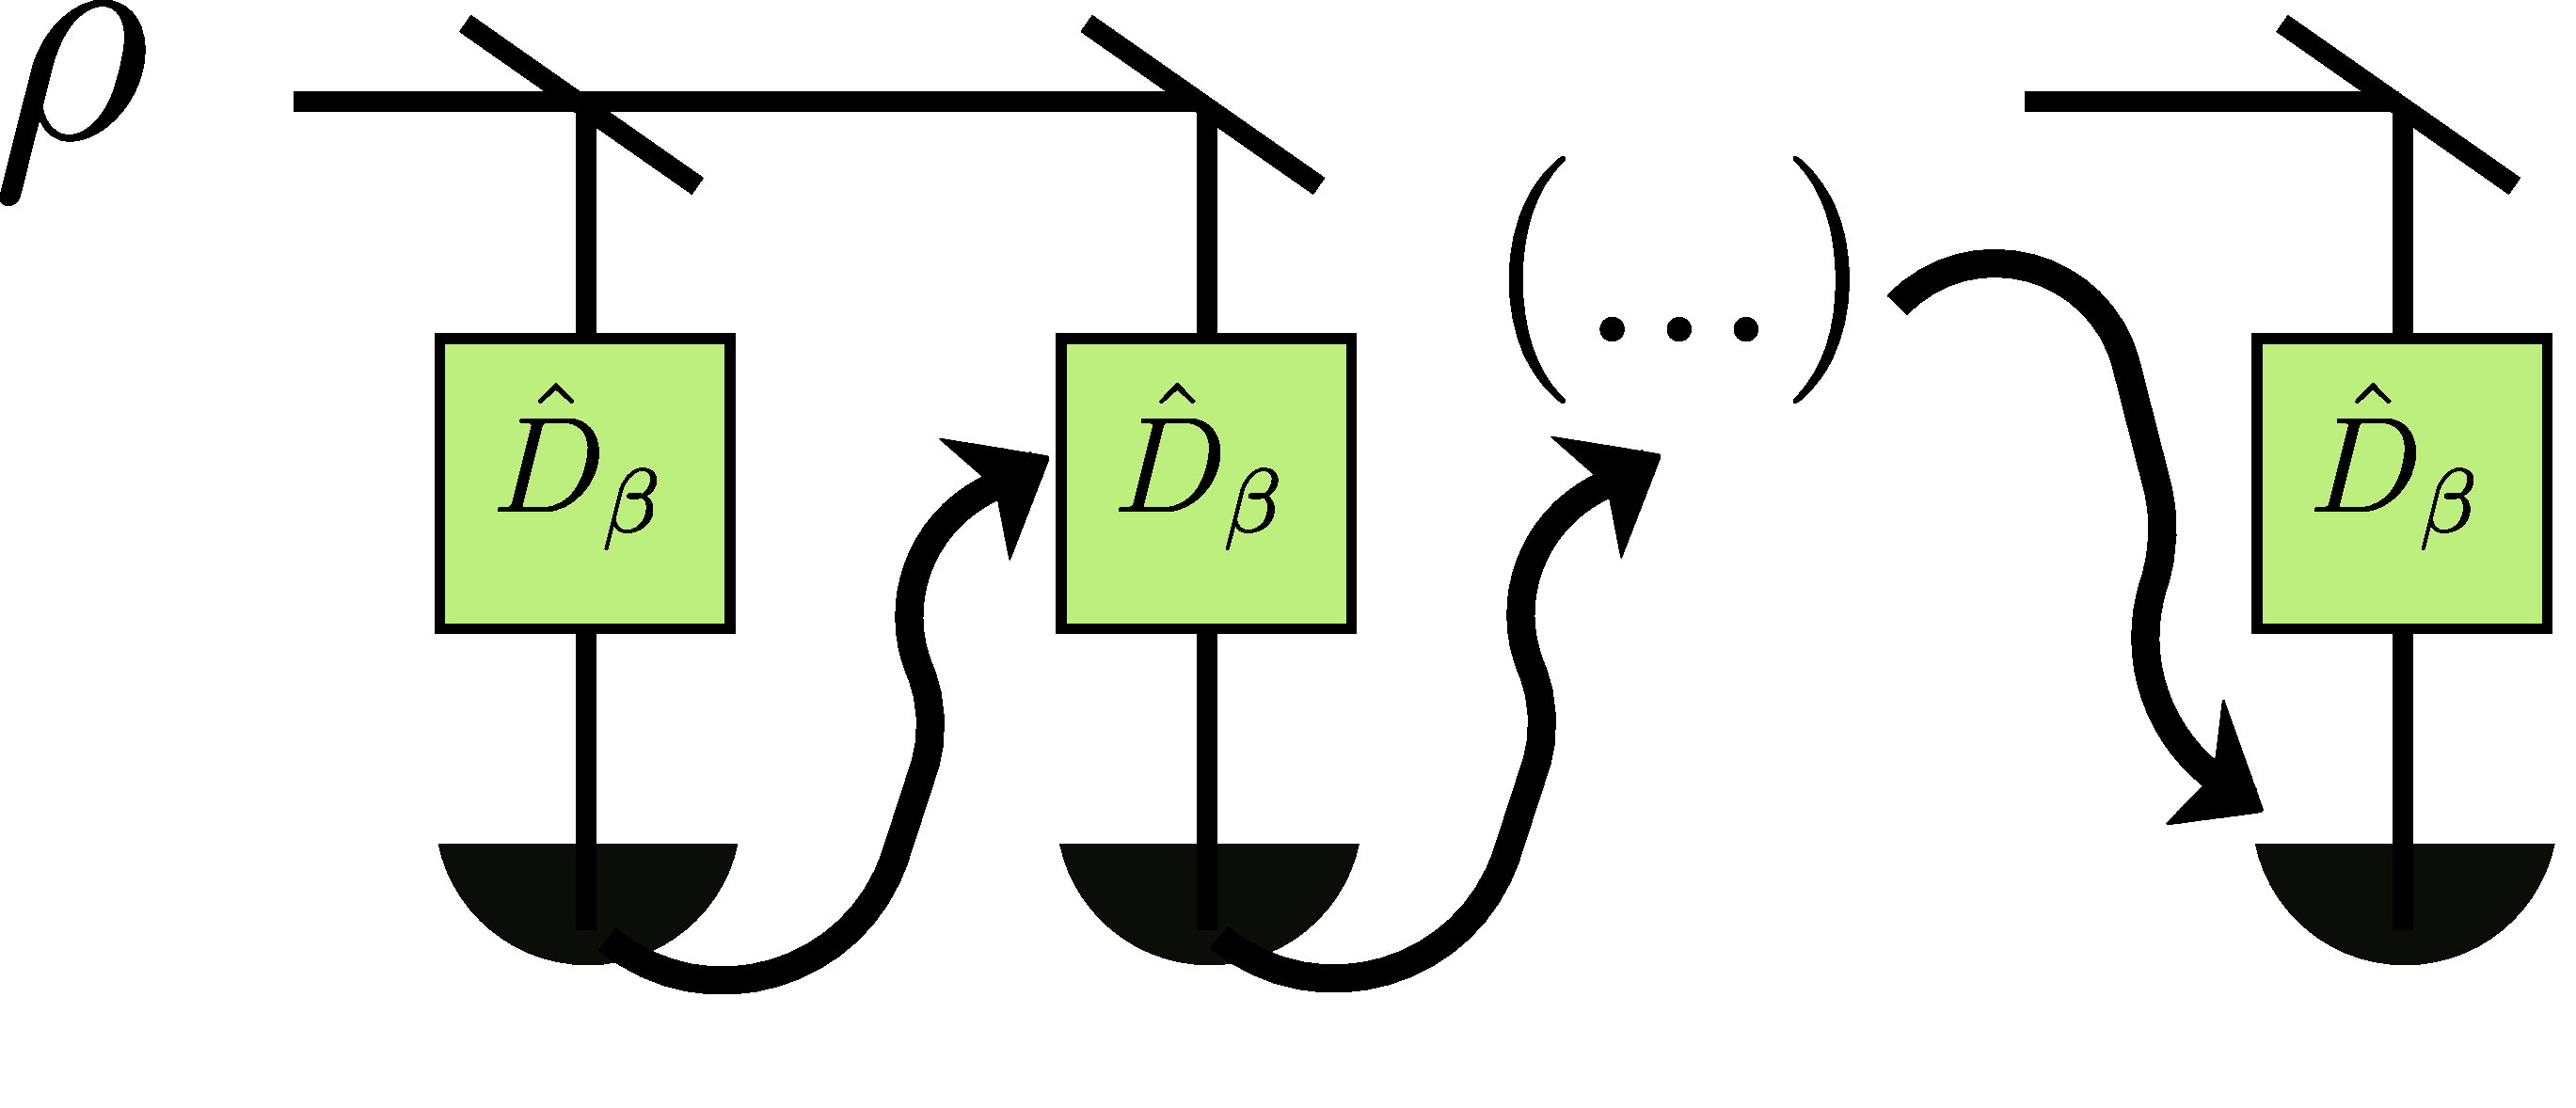
\includegraphics[width=.8\textwidth]{Figures/313/dolinar_receiver.pdf}
    \caption{We show a Dolinar-like receiver. For an infinite sequence measurements and feedforward operations, such a scheme attains the Helstrom bound for binary coherent-state discrimination.}
    \label{fig:313dolinar_setup}
\end{figure}
We note that for $L=1$ we recover the optimized-Kennedy receiver. However, because of its structure consisting on $L$ processing \textit{layers} $\ell=0,\cdots,L$, Dolinar receiver is considerably more complex than the Kennedy one. Specifically, for each layer $\ell<L$, the following operations are applied:
\begin{enumerate}
\item The input signal $\ket{\alpha}$ (or equivalently $\ket{-\alpha}$) is split on a BS of transmissivity $\theta$, effectively extracting a fraction $1-\theta$ of the energy for detection. The BS transforms the input signal and vacuum states as
\begin{equation}
\ket{\alpha}\ket{0}\mapsto\ket{\alpha\sqrt{\theta}}_{\rm tr}\ket{\alpha\sqrt{1-\theta}}_{\rm ref},
\end{equation}
Note that the BS adds a phase to the second mode, which we assumed corrected via a proper phase-shifter not shown in the figure.
\item The reflected part of the signal undergoes a displacement operation $\Dis{\beta}$. Such operation is realizable via interference with a strong coherent signal on a small-reflectivity BS, not shown in the figure. The resulting state is $\ket{\tilde{\alpha}(\beta,\theta)}_{\text{ref}}=\Dis{\beta}\ket{\alpha\sqrt{1-\theta}}_{\text{ref}}$.
\item\label{ops:end} The displaced signal is measured via a on/off photodetector, which detects no photon, i.e., outcome $o_{\ell+1} = 0$, with conditional probability
\begin{equation}\label{eq:313singLayProb}
p(o_{\ell+1}=0|\alpha,(\beta,\theta))=\abs{\braket{0}{\tilde{\alpha}(\beta,\theta)}_{\text{ref}}}^{2}=e^{-\abs{\tilde{\alpha}(\beta,\theta)}^{2}},
\end{equation}
and detects one or more photons, i.e., $o_{\ell+1}=1$, with probability $1-p(o_{\ell+1}=0|\alpha,(\beta,\theta))$.
\item The transmitted part of the signal enters layer $\ell+1$.
\end{enumerate}
Finally, the last processing layer $\ell=L$ consists in elaborating a guess $\hat{k}$ of the true hypothesis $k$, based on previous measurement outcomes and parameter choices.

Similar to $\beta$-Kennedy receivers, Dolinar-like receivers are parametrized by the displacements $\Dis{\beta}$. Nevertheless, the complexity is considerably higher: while $L$ displacement operations should be performed per signal detection, the feed-forward conditioning non-trivally enlarges the optimization landscape to $2^{L}-1$ possible values.

In addition, we shall now adopt the control-theory mindset introduced in Sec.~\ref{sec:1_rl},%\footnote{We will indistinctly talk about optimal control theory and reinforcement learning, while both fields come from different communities, they are faces of the same coin.} introduced in Sec.~\ref{ssec:rlcoh_kennedyreceiver}. Here,
and think of the displacements $\Dis{\beta_\ell}$ and attenuations $\theta_\ell$ as \textit{actions} $a_{\ell}$ performed on the signal.

Under these definitions, let us now study the success probability associated to a Dolinar-like receiver. For an initial coherent state $\ket{\alpha}$, the input state at the $\ell$-th layer is $\ket{\alpha_{\ell}}=\ket{\alpha\sqrt{\theta_{0}\cdots\theta_{\ell-1}}}$. In principle, we can use all the past history defined as
\equ{h_{\ell}=(a_{0},o_{1},\cdots,a_{\ell-1}),}
with $h_{0}=\emptyset$, to decide the next value of $(\beta,\theta)$ and the final guess. We label them compactly as $a_\ell(h_{\ell})=(\beta_{h_{\ell}},\theta_{h_{\ell}})$ and $a_{L}(h_{L})=\hat{k}$, omitting the label $\ell$ or the dependence on $h_{\ell}$ when it is clear from the context.

Hence, the average success probability of the $L$-Dolinar receiver, \textit{calibrated} under actions $\{a_\ell\}$, and averaged out over all possible outcomes' sequences $o_{1:L}=(o_{1},\cdots,o_{L})$ can be written as
\begin{equation}\label{eq:psdol}
P_{s}(\alpha,\{a_\ell\})=\sum_{o_{1:L}} \prod_{\ell=1}^{L}p(o_{\ell}|\alpha^{(k)},a(h_{\ell})) \; p_{k}\Big|_{k=a(h_{L})},
\end{equation}
Here, the configuration $\{a_{\ell}\}$ is the total set of actions over all histories, and we have written the conditional probability of the sequence of outcomes $o_{1:L}$ as a product of single-layer conditional probabilities, \textit{e.g.} Eq.\eqref{eq:313singLayProb}. In particular, we aim to optimize this success probability over the available actions of the receiver, and this value will denote as
\begin{equation}\label{eq:32OptSuc}
  P_{*}^{(L)}(\alpha) = \underset{\llaves{a_{\ell}}}{\text{ max }} P_s(\alpha, \llaves{a_\ell}).
\end{equation}
We will omit the dependence on $L$ whenever it is clear from the context.

The importance of the Dolinar receiver is that \textit{it is known to attain the Helstrom bound} in the limit of many layers, \textit{i.e.} $L\rightarrow \infty$, provided that the optimal actions are performed. However, before discussing such optimality and the structure of the receiver further, we will comment on an alternative formulation of this receiver.

\subsection{Time-domain Dolinar receiver $\&$ optimality}\label{ssec:tdol}
\begin{figure}[t!]
    \centering
    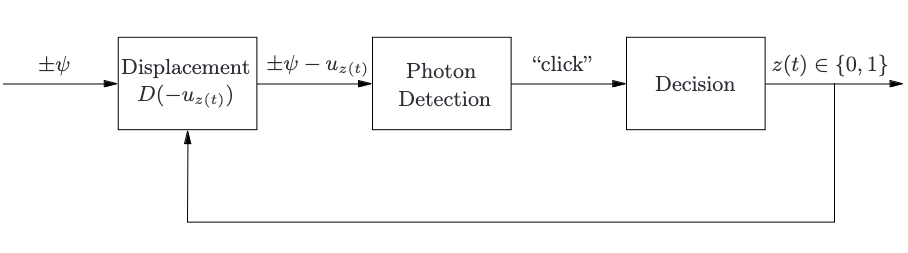
\includegraphics[width=1.\textwidth]{Figures/dolianr_cont.png}
    \caption{We show the original proposal of the Dolinar receiver, which works in continuous-time. This image is taken from Ref.~\cite{revisiting2011Assalini}. Instead of splitting the coherent-state in space by a beam-splitter array, we here have the signal spread in time, as explained in the main-body. The $\ell$-dependence in the conditional displacements is now translated into a time-dependence for $u(t)$, which in turn depends on the parity of the measurement outcomes as captured by the function $z(t)$. After the pulse-duration $T$, a decision for the phase of the coherent state is done via the function $z(T)$.}
    \label{fig:dolinar_cont}
\end{figure}
While we have introduced Dolinar receiver in the spatial-domain, its original formulation was done in the continuous-time domain~\cite{Dolinar}. The two formulations are related to each other by the equivalence between continuous-time photon-counting procesess and a (sufficiently-large) sequence of lossless beam-splitters and photon-detectors, as shown in Ref.~\cite{quasicontinuous}.

In the time-domain picture, the coherent state $\ket{\pm \alpha}$ is understood as a travelling-mode, and given by the field $\psi(t) = \pm \psi e^{\ii \omega t}$, where $\omega$ is the optical frequency and $|\alpha|^2 = \int_0^T |\psi(t)|^2dt = \psi^2 T$, with $T$ the total duration of the pulse. At each time $t$, the receiver shifts the incoming-field by a value $u_{z(t)}(t)$, and measures it by a photon-detector, as depicted in Fig.~\ref{fig:dolinar_cont}. Such measurement is assumed to be carried out very fast, leading only to binary outcomes (click or no click), which defines a so-called
\textit{compound Poisson process}. As shown in Dolinar's PhD thesis, the most-likely hypothesis $k$ is given by the parity of the sum of the outcomes obtained up to time $t$, and this determines the binary value $z(t)$ that controls the nature of the displacements to be done at consecutive times. The optimal shape of the pulses $u_{z(t)}(t)$ and of the success-probability of this scheme was originally derived in Ref.~\cite{Dolinar} by performing a dynamic programming optimization of the likelihood-ratio; in turn, he was able to show that the receiver attains the Helstrom bound. %However, following his approach can be painful, and we refer the interested reader to Refs.~\cite{Geremia2004,revisiting2011Assalini} for more compact proofs of the optimality.

In this line, the optimality of Dolinar receiver can also be proved in the spatial-domain (\textit{e.g.} the array of beam-splitters and conditional displacements) as follows. With sufficiently many measurement layers, say $L$, the coherent state will be splitted into $L$ copies, each having a very low intensity. From here, we can recall the results of Ref.~\cite{Acin2005Multi}, namely that the optimal discrimination between multiple copies of two pure quantum states can be achieved by a sequential strategy, in the assymptotic case of many copies. This strategy consists on a local projective measurement that is optimized at each step according to the most likely hypothesis; most notably the global measurement optimization problem is solved by an adaptive-local measurement, which hinges on bayesian updating the prior probabilities of each hypothesis after each measurement result. Such strategy is shown to achieve the Helstrom bound, and it can readily be applied to the $L$ copies of the attenuated coherent-state. In Ref.~\cite{revisiting2011Assalini} it was shown that, following this approach, the optimal adaptive measurement coincides with the Dolinar receiver, in the binary coherent-state discrimination problem. Also, let us mention that an alternative proof of Dolinar receiver's optimality is given in Ref.~\cite{Takeoka2005}

\bigskip
However, in practical experimental scenarios it is not possible to perform a large number of measurement layers. Such constraint is justified by \textit{(i)} the experimental feasibility of constructing the receiver, and \textit{(ii)} the noise accumulation at every layer.

Moreover, noise might even accumulate with the number of layers, as it happens with one of the most common sources of photon-detectors noise, the dark counts. Here, a click appears in the detector even when measuring the vacuum. Moreover, optimality of Dolinar receiver also requires the feed-forward operation to act before the signal reaches the next measurement layer. However, measuring and classical post-processing do take some time, and this delay is in practice modelled by including losses in between each measurement layer~\cite{sychLeuchs}.

From our previous discussion, it might seem that we are heading towards a paradigm where a set of suggestions is given to the experimentalist, with the optimizing actions in Eq.~\ref{eq:32OptSuc} essentially constituting the recipe to follow. This paradigm is actualy followed in Chapter~\ref{chapter:VANS}, where several cost-minimizing quantum circuits are discovered using our VAns algorithm, which is shown to work under several noise-models. While our experimental simulations should be realistic as possible, the usefulness of the recipe we provide will ultimately depend on how accurate can reality be modeled.

On the contrary, we will here tackle the situation from a different angle, and adapt to reality on the fly. This is the radical and experimentally-centered approach taken in this Chapter. To this end, a reinforcement-learning agent is faced towards the discrimination experiment, and asked to optimize its Dolinar-like receiver by having only access to an answer: \textit{yes/no}, a binary value standing for the correctness of its guess.
